\graphicspath{{chapters/chapter2/imgs/}}

\chapter{Sposoby generowania narracji}\label{chapter:ch2}

W poprzednich sekcjach omówiona została historia oraz wykorzystywane w grach komputerowych rodzaje
narracji. W każdym z tych elementów istnieje jeden element wspólny: to ludzie odpowiadają za tworzenie
narracji, odpowiednie jej planowanie i prezentowanie odbiorcy. Związane z tym są oczywiście olbrzymie
koszty oraz duży nakład czasu poświęcony przez pracowników. Biorąc pod uwagę terminy stale goniące
producentów gier, nic dziwnego, że pewne zaplanowane fragmenty fabularne nie znajdują miejsca w końcowym
produkcie. Z tego względu, patrząc na postępujący rozwój technologiczny, nasuwa się pytanie ---
czy da się zarządzać narracją w grze komputerowej w sposób automatyczny? W ramach tej sekcji
przedstawione zostaną znane rozwiązania z dziedziny sztucznej inteligencji pomagające w kreowaniu fabuły
oraz nakreślony zostanie potencjał w tej sferze dużych modeli językowych.

\section{Wykorzystanie algorytmów sztucznej inteligencji do kreowania narracji}\label{section:ch2_1}

Mówiąc o ogólnym wykorzystaniu algorytmów sztucznej inteligencji można cofnąć się do bardzo prostych
rozwiązań wykorzystanych np. w "Pong" (Patrz sekcja \ref{subsection:ch1_1_2}), do technik generowania
proceduralnego (zwłaszcza poziomów) czy też do systemów rankingowych (np. system TrueSkill). Jako, że
nie są to metody stricte powiązane z narracją to nie zostaną one opisane bardziej szczegółowo.
Przedstawione natomiast będą kluczowe obszary wykorzystywane w grach: częściowo-uporządkowane planowanie
(ang. \textit{POP} - partially-ordered planning), modelowanie doświadczeń gracza (ang. \textit{PEM} -
player experience modelling), przetwarzanie języka naturalnego (ang. \textit{NLP} - natural language
processing), postać niegrywalna (ang. \textit{NPC} - non-playable character), proces decyzyjny Markowa
(ang. \textit{MDP} - Markov decision process).

\subsubsection*{POP (Partially-ordered planning)}

Planowanie częściowo-uporządkowane jest skierowanym grafym acyklicznym, gdzie węzły są operacjami
(inaczej nazywanymi akcjami), które po wywołaniu zmieniają stan świata. Krawędzie przedstawiają
relacje przyczynowe i czasowe pomiędzy akcjami. Powiązanie przyczynowe $a_{i} \rightarrow^{c}a_{j}$
oznacza, że wykonanie akcji $a_{i}$ zmieni stan warunku $c$ na prawdziwy w świecie fabuły, a co za
tym idzie akcja $a_{j}$ zależna od tego warunku będzie możliwa do wykonania. Powiązanie czasowe
przedstawia ograniczenie porządkowe pomiędzy operacjami, gdzie jedna operacja musi być wykonana przed
inną\cite{game_ai_storytelling}. Przykładowa struktura fabularna zrealizowana za pomocą planowania
częściowo-uporządkowanego została przedstawiona na rysunku \ref{fig:ch2_1_pop}.

\begin{figure}[h]
    \centering
    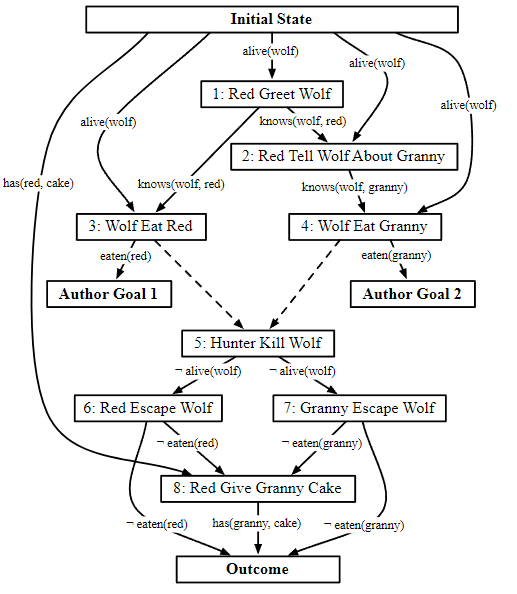
\includegraphics[width=0.5\textwidth]{ch2_1_pop.png}
    \caption{Fabuła "Czerwonego Kapturka" zapisana za pomocą POP}
    \label{fig:ch2_1_pop}
\end{figure}

Za pomocą tej techniki kreować można rozbudowane plany fabularne, które mogą ulegać zmianie na
podstawie akcji podejmowanych przez gracza czy zmian zachodzących w świecie gry. Odpowiednie algorytmy
przeszukiwania nazywane \textit{"plannerami"} rozwiązują problem planowania, tzn. mając dany stan
świata, pewne atomowe akcje możliwe do wykonania przez grającego oraz założony cel, znajdują
odpowiednią sekwencję operacji, które doprowadzą do osięgnięcia tegoż celu\cite{game_ai_storytelling}.

Podstawowym problemem pojawiającym się przy wykorzystaniu metody POP jest to, że zarówno gracz jak i
potencjalnie inne niegrywalne postacie, mogą być zdolne do wywołania akcji w świecie gry, która
zagraża dalszemu przebiegowi fabularnemu zgodnego z planem\cite{characters_and_directors}. Wtedy
stosowane są odpowiednie techniki naprawcze, które prowadzą do mniej lub bardziej doskonałych rozwiązań.

\subsubsection*{PEM (Player experience modelling)}

Modelowanie doświadczeń gracza polega na zbieraniu danych behawioralnych czy też wydajnościowych
(punkty, czas, decyzje) ze względu na rozgrywkę za pomocą wielu modalności: mowy gracza, obrazów
(śledzenie ruchów ciała, mimiki twarzy, gałek ocznych) czy też sygnałów fizjologicznych (puls czy
przewodność skóry). Pomiar sygnałów fizjologicznych jest oczywiście problematyczny ze względu na
wykorzystanie dodatkowego sprzętu a zarazem inwazyjność przeszkadzającą w swobodnej rozgrywce
\cite{reusable_game_ai}.

W ramach tego obszaru sztuczna inteligencja objawia się zazwyczaj pod postacią sieci neuronowych czy
też drzew decyzyjnych, które pozwalają dokonywać klasyfikacji w zakresie\cite{reusable_game_ai}:

\begin{itemize}
    \item rozpoznawania emocji grającego - w ramach anagażujących systemów dialogowych
    \item balansowania rozgrywki - tak by gracz nie odczuwał frustracji ze względu na zbyt wysoki poziom
          trudności a zarazem by nie doznawał nudy ze względu na zbyt prostą rozgrywkę
    \item oceniania umiejętności gracza - do prowadzenia badań w sposób ukryty
\end{itemize}

\subsubsection*{NLP (Natural language processing)}

Przetwarzanie języka naturalnego jest dziedziną w obrębie sztucznej inteligencji, która zajmuje się
zrozumieniem, interpretacją i manipulacją ludzkiego języka\cite{reusable_game_ai}. W ramach gier
komputerowych pozwala to graczowi poruszać się po świecie czy też komunikować z innymi postaciami NPC
w sposób zarówno naturalny (zamiast wchodzenia w interakcję z odpowiednimi interfejsami) jak i dość
otwarty (na tyle na ile dany system jest w stanie przetwarzać odpowiednie frazy).

Z podstaw przetwarzania języka naturalnego korzystały tytuły realizowane w konwencji interaktywnej
fikcji, takie jak "Otchłań" (Patrz sekcja \ref{subsection:ch1_3_2}). Pozwalają one graczowi za pomocą
określonego zestawu komend poruszać się i wchodzić w interakcję z całym światem gry.

Związane z tą dziedziną są duże modele językowe, które potrafią operować językiem naturalnym.
Ich bardziej szczegółowy opis będzie przedstawiony w sekcji \ref{section:ch2_2}.

\subsubsection*{NPC (Non-playable character)}

Postacie niegrywalne to wszelkie jednostki czy postacie, z którymi gracz może wchodzić w
interakcję lub dostrzegać ich autonomiczne poruszanie w świecie. Mogą to być statyczne byty,
które usytuowane są w jednym określonym miejscu i mają na celu dawać grającemu zadania czy też
informacje o świecie gry. Z drugiej strony wszelkie jednostki, z którymi gracz walczy również
podlegają pod tę definicję. Forma postaci niegrywalnych, tak jak i w literaturze, nie jest
istotna, gdyż bohaterem może być zarówno człowiek jak i zantropomorfizowane zwierzę czy rzecz.

NPC pojawiły się w grach z początkiem lat 90-tych. Oparte były przede wszystkim na zpredefiniowanych
skryptach i drzewach decyzyjnych\cite{storytelling_through} (współcześnie nadal wiele postaci jest
opartych o te rozwiązania) \cite{from_pong_to_narrative}.

Wraz z rozwojem technologicznym twórcy gry mają możliwość przeznaczenia więcej mocy obliczeniowej
na wiarygodne dla gracza postacie NPC. Związane jest to z dokładniejszymi modelami i animacjami
postaci ale również z bardziej zaawansowanymi wzorcami zachowania. Producenci zaczęli wykorzystywać
od lat 2010 w tym celu techniki uczenia maszynowego oraz głębokiego nauczania
\cite{from_pong_to_narrative}. Pozwala to przeciwnikom (czy też sprzymierzeńcom) gracza
dostosowywać się do sposobu prowadzenia przez niego rozgrywki. Współczesne tytuły takie jak
"Read Dead Redemption 2" czy "The Last of Us Part II" wykorzystują głębokie sieci neuronowe do
budowania postaci NPC\cite{from_pong_to_narrative}.

\subsubsection*{MDP (Markov decision process)}

Łańcuch Markowa jest stochastycznym modelem opisującym ciąg możliwych zdarzeń, w którym
prawdopodobieństwo każdego zdarzenia zależy jedynie od wyniku poprzedniego. Rozróżniane one
są dodatkowo ze względu na dyskretne lub ciągłe momenty czasowe, w których następuje zmiana
stanów. Proces decyzyjny Markowa (MDP) jest zasadniczo rozszerzeniem łańcuchów Markowa ---
różnicę stanowi dodanie akcji (które pozwalają na podejmowanie decyzji) oraz nagród otrzymywanych
po przejściu z jednego stan w drugi. Jeżeli dla każdego stanu istnieje tylko jedna akcja i
wszystkie nagrody są jednakowe, to proces decyzyjny Markowa upraszcza się do łańcucha Markowa.

\begin{figure}[h]
    \centering
    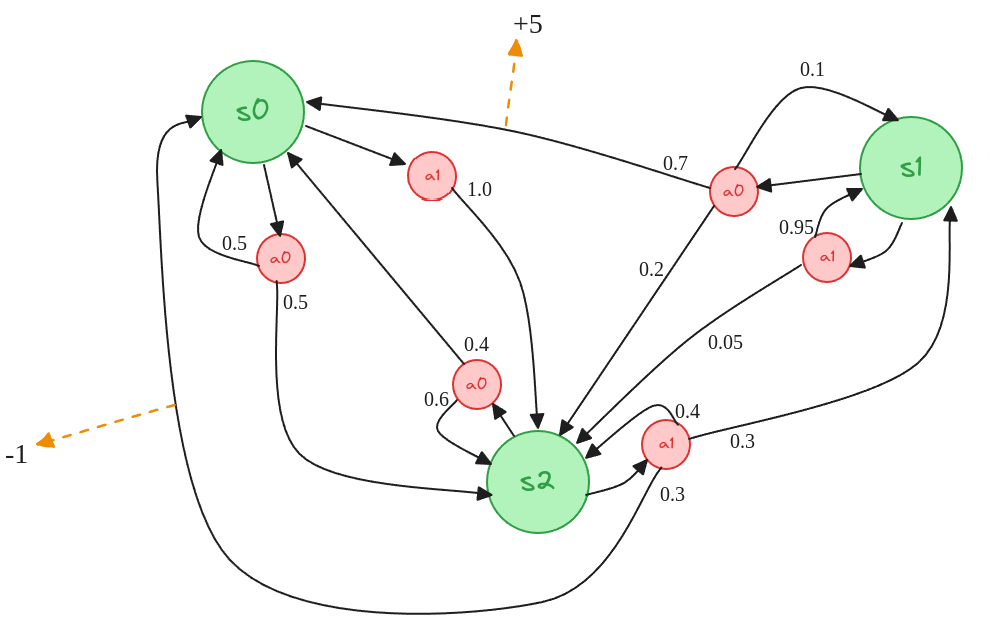
\includegraphics[width=0.8\textwidth]{ch2_1_mdp.png}
    \caption{Przykładowy proces decyzyjny Markowa}
    \label{fig:ch2_1_mdp}
\end{figure}

Na powyższym rysunku przedstawiony został przykładowy proces decyzjny Markowa z trzema stanami (zielone
kółka), dwiema akcjami (czerwone kółka) oraz dwiema nagrodami (pomarańczowe strzałki). Model MDP może
być wykorzystany w ramach generowania treści gier komputerowych do budowania zadań dla gracza,
przykładowo dla gry kucharskiej baza składników może być ułożona w odpowiednie łańcuchy Markowa, tak
by bardziej pasujące do siebie składniki miały większe prawdopodobieństwo bycia wspólnie wybranym
\cite{ammanabrolu2020automated}.

Proces może być dodatkowo wykorzystany w proceduralnym generowaniu treści czy świata dla gracza.
Zakładając, że to gracz jest \textit{"agentem"} podejmującym akcje w świecie gry (które są jawnie
zdefiniowane przez twórców), doprowadza on do zmiany stanu świata co jest idealnie reprezentowane
przez proces decyzyjny Markowa\cite{automated_planning}.

\subsubsection*{Przykład wykorzystania - "Façade"}

"Façade" (2005) to tytuł, który próbował złamać znany do tamtej pory podział na narrację liniową czy też
rozgałęziającą się, na rzecz w pełni interaktywnej historii kontrolowanej przez gracza. Jest to
trójwymiarowa gra czasu rzeczywistego przedstawiona w formie jednego aktu. Narracja koncentruje się
wokół Grace i Tripa, małżeństwa po trzydziestce, które zaprasza gracza na drinka. Gracz nie wie, że ich
małżeństwo znajduje się na grząskim gruncie, a tego wieczoru wszystkie ich małżeńskie problemy wyjdą na
jaw. To, w jaki sposób ich związek się rozpadnie, a także ostateczny związek gracza z Grace i Tripem,
zależy od interakcji gracza ze światem. Gracz angażuje się poprzez poruszanie się po środowisku,
manipulowanie przedmiotami i, co najważniejsze, poprzez dialogi w języku naturalnym\cite{1024751}.

Twórcy na potrzebę "Façade" stworzyli własny język ABL (\textit{"A Behavior Language"} - z ang. język
zachowań). Stanowi on pewnego rodzaju połączenie drzew decyzjnych i procesów decyzjnych Markowa
wspomnianych wcześniej. Programy ABL są zorganizowane jako zbiór zachowań, które mogą być procesowane
sekwencyjnie lub równolegle. Dodatkowo, zachowania mogą mieć narzucone określone wymagania by
mogły one się odbyć, a w zależności od powodzenia lub porażki w realizacji zachowania świat gry
może zostać odpowiednio zmieniony.

\section{Wykorzystanie dużych modeli językowych (LLM) do kreowania narracji}\label{section:ch2_2}

Bla bla bla duże modele językowe są coraz popularniesze i coraz lepsze, więc zaczynają być
wykorzystywane w coraz więcej miejscach. W tej sekcji przedstawiona zostanie krótka charakterystyka
dużych modeli językowych, potencjalne formy ich wykorzystania oraz przykład praktyczny.

\subsubsection*{Definicja i charakterystyka dużych modeli językowych}

Bla bla bla...

\subsubsection*{Potencjalne struktury wykorzystania dużych modeli językowych}

Bla bla bla...

\subsubsection*{Przykład zastosowania dużych modeli językowych}

Tutaj będzie o QuestVille i może o Inworld.AI czy coś...